\begin{figure}[H]
    \centering




    \tikzset{every picture/.style={line width=0.75pt}} %set default line width to 0.75pt

    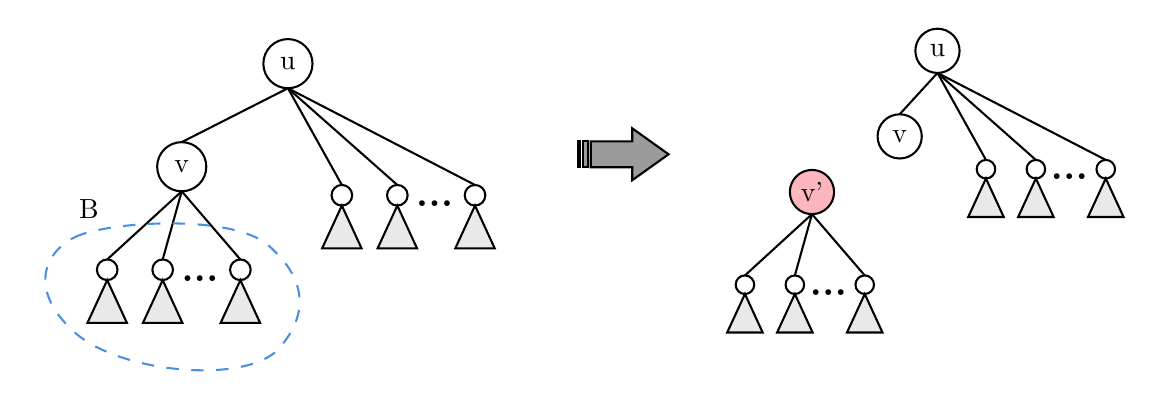
\begin{tikzpicture}[x=0.75pt,y=0.75pt,yscale=-1,xscale=1]
        %uncomment if require: \path (0,476); %set diagram left start at 0, and has height of 476

        %Shape: Ellipse [id:dp7890393065744103]
        \draw  [fill={rgb, 255:red, 255; green, 255; blue, 255 }  ,fill opacity=1 ] (124.52,36.84) .. controls (124.52,30.3) and (129.83,25) .. (136.36,25) .. controls (142.9,25) and (148.2,30.3) .. (148.2,36.84) .. controls (148.2,43.38) and (142.9,48.68) .. (136.36,48.68) .. controls (129.83,48.68) and (124.52,43.38) .. (124.52,36.84) -- cycle ;
        %Shape: Ellipse [id:dp618735643725828]
        \draw  [fill={rgb, 255:red, 255; green, 255; blue, 255 }  ,fill opacity=1 ] (73.35,86.49) .. controls (73.35,79.95) and (78.65,74.65) .. (85.19,74.65) .. controls (91.72,74.65) and (97.03,79.95) .. (97.03,86.49) .. controls (97.03,93.03) and (91.72,98.33) .. (85.19,98.33) .. controls (78.65,98.33) and (73.35,93.03) .. (73.35,86.49) -- cycle ;
        %Shape: Ellipse [id:dp4771904397826303]
        \draw   (44.32,136.14) .. controls (44.32,133.4) and (46.54,131.18) .. (49.28,131.18) .. controls (52.03,131.18) and (54.25,133.4) .. (54.25,136.14) .. controls (54.25,138.88) and (52.03,141.11) .. (49.28,141.11) .. controls (46.54,141.11) and (44.32,138.88) .. (44.32,136.14) -- cycle ;
        %Shape: Triangle [id:dp553752456661303]
        \draw  [fill={rgb, 255:red, 233; green, 233; blue, 233 }  ,fill opacity=1 ] (49.28,141.11) -- (58.78,161.73) -- (39.78,161.73) -- cycle ;

        %Shape: Ellipse [id:dp4582325504788667]
        \draw   (71.05,136.14) .. controls (71.05,133.4) and (73.28,131.18) .. (76.02,131.18) .. controls (78.76,131.18) and (80.98,133.4) .. (80.98,136.14) .. controls (80.98,138.88) and (78.76,141.11) .. (76.02,141.11) .. controls (73.28,141.11) and (71.05,138.88) .. (71.05,136.14) -- cycle ;
        %Shape: Triangle [id:dp5979831512805434]
        \draw  [fill={rgb, 255:red, 233; green, 233; blue, 233 }  ,fill opacity=1 ] (76.02,141.11) -- (85.52,161.73) -- (66.52,161.73) -- cycle ;

        %Shape: Ellipse [id:dp2963506198722945]
        \draw   (108.48,136.14) .. controls (108.48,133.4) and (110.71,131.18) .. (113.45,131.18) .. controls (116.19,131.18) and (118.41,133.4) .. (118.41,136.14) .. controls (118.41,138.88) and (116.19,141.11) .. (113.45,141.11) .. controls (110.71,141.11) and (108.48,138.88) .. (108.48,136.14) -- cycle ;
        %Shape: Triangle [id:dp6725407515322526]
        \draw  [fill={rgb, 255:red, 233; green, 233; blue, 233 }  ,fill opacity=1 ] (113.45,141.11) -- (122.95,161.73) -- (103.95,161.73) -- cycle ;

        %Shape: Circle [id:dp18476563967542958]
        \draw   (157.37,100.24) .. controls (157.37,97.5) and (159.59,95.28) .. (162.34,95.28) .. controls (165.08,95.28) and (167.3,97.5) .. (167.3,100.24) .. controls (167.3,102.98) and (165.08,105.21) .. (162.34,105.21) .. controls (159.59,105.21) and (157.37,102.98) .. (157.37,100.24) -- cycle ;
        %Shape: Triangle [id:dp466803100468395]
        \draw  [fill={rgb, 255:red, 233; green, 233; blue, 233 }  ,fill opacity=1 ] (162.34,105.21) -- (171.84,125.83) -- (152.83,125.83) -- cycle ;

        %Shape: Circle [id:dp5261729680381961]
        \draw   (184.11,100.24) .. controls (184.11,97.5) and (186.33,95.28) .. (189.07,95.28) .. controls (191.81,95.28) and (194.04,97.5) .. (194.04,100.24) .. controls (194.04,102.98) and (191.81,105.21) .. (189.07,105.21) .. controls (186.33,105.21) and (184.11,102.98) .. (184.11,100.24) -- cycle ;
        %Shape: Triangle [id:dp20443302728402402]
        \draw  [fill={rgb, 255:red, 233; green, 233; blue, 233 }  ,fill opacity=1 ] (189.07,105.21) -- (198.57,125.83) -- (179.57,125.83) -- cycle ;

        %Shape: Circle [id:dp720535105016272]
        \draw   (221.53,100.24) .. controls (221.53,97.5) and (223.76,95.28) .. (226.5,95.28) .. controls (229.24,95.28) and (231.46,97.5) .. (231.46,100.24) .. controls (231.46,102.98) and (229.24,105.21) .. (226.5,105.21) .. controls (223.76,105.21) and (221.53,102.98) .. (221.53,100.24) -- cycle ;
        %Shape: Triangle [id:dp7645667177753481]
        \draw  [fill={rgb, 255:red, 233; green, 233; blue, 233 }  ,fill opacity=1 ] (226.5,105.21) -- (236,125.83) -- (217,125.83) -- cycle ;

        %Straight Lines [id:da07079731319780569]
        \draw    (85.19,98.33) -- (49.28,131.18) ;


        %Straight Lines [id:da17784879908658002]
        \draw    (85.19,98.33) -- (76.02,131.18) ;


        %Straight Lines [id:da15620515081223996]
        \draw    (85.19,98.33) -- (113.45,131.18) ;


        %Straight Lines [id:da8013781550577805]
        \draw    (136.36,48.68) -- (85.19,74.65) ;


        %Straight Lines [id:da945479179142265]
        \draw    (136.36,48.68) -- (162.34,95.28) ;


        %Straight Lines [id:da1078430250095277]
        \draw    (136.36,48.68) -- (189.07,95.28) ;


        %Straight Lines [id:da2224960955888713]
        \draw    (136.36,48.68) -- (226.5,95.28) ;


        %Shape: Polygon Curved [id:ds3544729654410035]
        \draw  [color={rgb, 255:red, 74; green, 144; blue, 226 }  ,draw opacity=1 ][dash pattern={on 4.5pt off 4.5pt}] (33.62,120.48) .. controls (48.9,112.84) and (109.25,109.02) .. (126.82,124.3) .. controls (144.38,139.58) and (147.44,156.38) .. (132.16,173.95) .. controls (116.89,191.52) and (55.78,186.17) .. (33.62,166.31) .. controls (11.47,146.45) and (18.35,128.12) .. (33.62,120.48) -- cycle ;
        %Shape: Ellipse [id:dp6954675899235474]
        \draw  [fill={rgb, 255:red, 255; green, 255; blue, 255 }  ,fill opacity=1 ] (438.66,30.65) .. controls (438.66,24.77) and (443.43,20) .. (449.31,20) .. controls (455.19,20) and (459.96,24.77) .. (459.96,30.65) .. controls (459.96,36.53) and (455.19,41.3) .. (449.31,41.3) .. controls (443.43,41.3) and (438.66,36.53) .. (438.66,30.65) -- cycle ;
        %Shape: Ellipse [id:dp2597907901086436]
        \draw  [fill={rgb, 255:red, 253; green, 181; blue, 190 }  ,fill opacity=1 ] (378.19,98.68) .. controls (378.19,92.79) and (382.96,88.03) .. (388.84,88.03) .. controls (394.72,88.03) and (399.49,92.79) .. (399.49,98.68) .. controls (399.49,104.56) and (394.72,109.33) .. (388.84,109.33) .. controls (382.96,109.33) and (378.19,104.56) .. (378.19,98.68) -- cycle ;
        %Shape: Ellipse [id:dp5664348554601168]
        \draw   (352.08,143.34) .. controls (352.08,140.87) and (354.08,138.87) .. (356.55,138.87) .. controls (359.01,138.87) and (361.01,140.87) .. (361.01,143.34) .. controls (361.01,145.81) and (359.01,147.81) .. (356.55,147.81) .. controls (354.08,147.81) and (352.08,145.81) .. (352.08,143.34) -- cycle ;
        %Shape: Triangle [id:dp7826763983443301]
        \draw  [fill={rgb, 255:red, 233; green, 233; blue, 233 }  ,fill opacity=1 ] (356.55,147.81) -- (365.09,166.36) -- (348,166.36) -- cycle ;

        %Shape: Ellipse [id:dp19804184401026292]
        \draw   (376.13,143.34) .. controls (376.13,140.87) and (378.13,138.87) .. (380.6,138.87) .. controls (383.06,138.87) and (385.06,140.87) .. (385.06,143.34) .. controls (385.06,145.81) and (383.06,147.81) .. (380.6,147.81) .. controls (378.13,147.81) and (376.13,145.81) .. (376.13,143.34) -- cycle ;
        %Shape: Triangle [id:dp1257939998917028]
        \draw  [fill={rgb, 255:red, 233; green, 233; blue, 233 }  ,fill opacity=1 ] (380.6,147.81) -- (389.14,166.36) -- (372.05,166.36) -- cycle ;

        %Shape: Ellipse [id:dp6791067615266415]
        \draw   (409.8,143.34) .. controls (409.8,140.87) and (411.8,138.87) .. (414.27,138.87) .. controls (416.73,138.87) and (418.73,140.87) .. (418.73,143.34) .. controls (418.73,145.81) and (416.73,147.81) .. (414.27,147.81) .. controls (411.8,147.81) and (409.8,145.81) .. (409.8,143.34) -- cycle ;
        %Shape: Triangle [id:dp05475095272330521]
        \draw  [fill={rgb, 255:red, 233; green, 233; blue, 233 }  ,fill opacity=1 ] (414.27,147.81) -- (422.81,166.36) -- (405.72,166.36) -- cycle ;

        %Shape: Ellipse [id:dp768190699412989]
        \draw   (468.21,87.68) .. controls (468.21,85.22) and (470.21,83.22) .. (472.67,83.22) .. controls (475.14,83.22) and (477.14,85.22) .. (477.14,87.68) .. controls (477.14,90.15) and (475.14,92.15) .. (472.67,92.15) .. controls (470.21,92.15) and (468.21,90.15) .. (468.21,87.68) -- cycle ;
        %Shape: Triangle [id:dp6281136326737822]
        \draw  [fill={rgb, 255:red, 233; green, 233; blue, 233 }  ,fill opacity=1 ] (472.67,92.15) -- (481.22,110.7) -- (464.13,110.7) -- cycle ;

        %Shape: Ellipse [id:dp5752389515789107]
        \draw   (492.26,87.68) .. controls (492.26,85.22) and (494.25,83.22) .. (496.72,83.22) .. controls (499.19,83.22) and (501.19,85.22) .. (501.19,87.68) .. controls (501.19,90.15) and (499.19,92.15) .. (496.72,92.15) .. controls (494.25,92.15) and (492.26,90.15) .. (492.26,87.68) -- cycle ;
        %Shape: Triangle [id:dp6106206395942142]
        \draw  [fill={rgb, 255:red, 233; green, 233; blue, 233 }  ,fill opacity=1 ] (496.72,92.15) -- (505.27,110.7) -- (488.18,110.7) -- cycle ;

        %Shape: Ellipse [id:dp6519300759581739]
        \draw   (525.92,87.68) .. controls (525.92,85.22) and (527.92,83.22) .. (530.39,83.22) .. controls (532.86,83.22) and (534.86,85.22) .. (534.86,87.68) .. controls (534.86,90.15) and (532.86,92.15) .. (530.39,92.15) .. controls (527.92,92.15) and (525.92,90.15) .. (525.92,87.68) -- cycle ;
        %Shape: Triangle [id:dp5630792182459539]
        \draw  [fill={rgb, 255:red, 233; green, 233; blue, 233 }  ,fill opacity=1 ] (530.39,92.15) -- (538.94,110.7) -- (521.85,110.7) -- cycle ;

        %Straight Lines [id:da06383027443032363]
        \draw    (388.84,109.33) -- (356.55,138.87) ;


        %Straight Lines [id:da9480602083613776]
        \draw    (388.84,109.33) -- (380.6,138.87) ;


        %Straight Lines [id:da6126344791679308]
        \draw    (388.84,109.33) -- (414.27,138.87) ;


        %Straight Lines [id:da9536257508469264]
        \draw    (449.31,41.3) -- (431.1,61.23) ;


        %Straight Lines [id:da776473603305027]
        \draw    (449.31,41.3) -- (472.67,83.22) ;


        %Straight Lines [id:da05961301813111186]
        \draw    (449.31,41.3) -- (496.72,83.22) ;


        %Straight Lines [id:da9006355028038635]
        \draw    (449.31,41.3) -- (530.39,83.22) ;


        %Shape: Ellipse [id:dp864192371104153]
        \draw  [fill={rgb, 255:red, 255; green, 255; blue, 255 }  ,fill opacity=1 ] (420.45,71.88) .. controls (420.45,66) and (425.22,61.23) .. (431.1,61.23) .. controls (436.98,61.23) and (441.75,66) .. (441.75,71.88) .. controls (441.75,77.76) and (436.98,82.53) .. (431.1,82.53) .. controls (425.22,82.53) and (420.45,77.76) .. (420.45,71.88) -- cycle ;
        %Striped Right Arrow [id:dp669887073415196]
        \draw  [fill={rgb, 255:red, 155; green, 155; blue, 155 }  ,fill opacity=1 ] (282.25,74.25) -- (302.25,74.25) -- (302.25,68) -- (319.75,80.5) -- (302.25,93) -- (302.25,86.75) -- (282.25,86.75) -- cycle ;\draw  [fill={rgb, 255:red, 155; green, 155; blue, 155 }  ,fill opacity=1 ] (276,74.25) -- (277.25,74.25) -- (277.25,86.75) -- (276,86.75) -- cycle ;\draw  [fill={rgb, 255:red, 155; green, 155; blue, 155 }  ,fill opacity=1 ] (278.5,74.25) -- (281,74.25) -- (281,86.75) -- (278.5,86.75) -- cycle ;

        % Text Node
        \draw (136.36,36.84) node  [align=left] {u};
        % Text Node
        \draw (85.19,86.49) node  [align=left] {v};
        % Text Node
        \draw (93.97,140.34) node  [align=left] {\textbf{{\Large ...}}};
        % Text Node
        \draw (207.02,104.44) node  [align=left] {\textbf{{\Large ...}}};
        % Text Node
        \draw (40.5,106.73) node  [align=left] {B};
        % Text Node
        \draw (449.31,30.65) node  [align=left] {u};
        % Text Node
        \draw (388.84,98.68) node  [align=left] {v'};
        % Text Node
        \draw (396.74,147.12) node  [align=left] {\textbf{{\Large ...}}};
        % Text Node
        \draw (512.87,91.46) node  [align=left] {\textbf{{\Large ...}}};
        % Text Node
        \draw (431.1,71.88) node  [align=left] {v};


    \end{tikzpicture}

    \caption{Steiner's Vertex for cut type B}\label{fig:steiner}
\end{figure}